% =============================================================================
%  Sección 1: Introducción
% =============================================================================

\section{Introducción}

\subsection{Objetivo del ensayo}

El presente ensayo tiene por objetivo evaluar los conceptos teóricos que se tienen en la movilidad del transporte público 
y contrastarlos con los hallazgos encontrados gracias al \termino{Modelo de la Higuera Evanescente \cite{Garibaldi2024VFT}} y 
el proyecto de Software libre \termino{Apimetro \cite{cabrera2025apimetro}}. Obteniendo un contraste en la base teórica 
y los estudios modernos y la realidad de la \zmvm.


\subsection{Definición de Conceptos}

En esta sección exploraremos los términos necesarios para entender el desarrollo de este ensayo. Teniendo como principal 
eje rector la sosteniblidad descrita en varios aspectos pero priorizando tres: Su factor social, ambiental y tecnológico. 
Para ello, se citarán diferentes estudios, artículos académicos o de divulgación científica y reportes obtenidos gracias 
al uso de la digitalización de la información.

\subsubsection{Introducción: La Evolución del Paradigma de Movilidad}
\label{subsubsec:evolucion-paradigma}

El fenómeno de la movilidad urbana en el siglo XXI ha dejado de ser una cuestión puramente técnica de ingeniería de 
tránsito para convertirse en el eje rector de la justicia socioespacial y la viabilidad ambiental de las metrópolis 
\cite{Litman2021}. En el contexto de la \zmvm, este cambio exige una transición profunda desde el paradigma tradicional 
del transporte hacia una visión sistémica e integrada de la movilidad humana.

\subsubsection{Evolución Conceptual: Del Transporte a la Movilidad}
\label{subsubsec:evolucion-transporte-movilidad}

La distinción epistemológica fundamental radica en el objeto de estudio. El \textbf{paradigma tradicional del transporte} 
se ha centrado históricamente en la gestión de flujos vehiculares, la capacidad de carga vial y la optimización de la 
velocidad del automóvil particular \cite{Garibaldi2024VFT, RedalycPeaton}. En contraste, el 
\textbf{paradigma contemporáneo de la movilidad sustentable} adopta un enfoque antropocéntrico basado en la 
\textbf{accesibilidad} de las personas y su capacidad para interactuar con el entorno urbano \cite{RamirezPacheco2025}. 
\\
Bajo esta visión del urbanismo posmoderno, el éxito de un sistema no se mide por el volumen de vehículos desplazados, sino 
por la capacidad de los ciudadanos para acceder a las oportunidades de la ciudad (empleo, salud, educación) de forma segura, 
eficiente y equitativa \cite{ITDP_Espacio}.

\subsubsection{Marco Legal y Ético: La Movilidad como Derecho Humano}
\label{subsubsec:marco-legal-etico}

Esta transición conceptual encuentra su blindaje jurídico en la reforma al \textbf{Artículo 4° Constitucional} del año 2020, 
que reconoce explícitamente el derecho de toda persona a la movilidad en condiciones de seguridad vial, accesibilidad, eficiencia, 
sostenibilidad e igualdad \cite{ConstitucionMex}.
\\
Como instrumento rector derivado de este mandato, la \textbf{Estrategia Nacional de Movilidad y Seguridad Vial (ENAMOV) 2023-2042} 
establece la hoja de ruta para los próximos veinte años, alineando las políticas nacionales con compromisos internacionales 
\cite{SEDATU2023}. La ENAMOV obliga a la implementación de una \textbf{Jerarquía de Movilidad} que sitúa al peatón y al ciclista 
en la cúspide del diseño vial, buscando revertir las desigualdades históricas en la distribución del espacio público \cite{SEDATU2023}.



\subsection{Enfoque en la Sostenibilidad y el Cambio Modal}
\label{subsec:sostenibilidad-cambio-modal}
 
La planeación estratégica del transporte público no puede disociarse de su dimensión
territorial y ambiental. \cite{ugur2025} señalan que la integración de los
diferentes modos de transporte público ---lograda mediante la evaluación sistemática
de la conectividad entre líneas y la creación de oportunidades efectivas de
transferencia--- incrementa la cobertura espacial de la red, mejora la accesibilidad
urbana, promueve el uso del transporte colectivo y contribuye a la reducción de
emisiones, al tiempo que garantiza la equidad social en la movilidad y ofrece opciones
de viaje más económicas. Desde esta perspectiva, la planeación estratégica tiene
como objetivo último facilitar el cambio modal del vehículo privado hacia el transporte
masivo, para lo cual la optimización de la red ---modelada como grafo--- es condición
necesaria.
 
\cite{moreno2023} enmarcan además este esfuerzo en el contexto de la soberanía
tecnológica del Estado, argumentando que el desarrollo de software propio de
asignación de tráfico, basado en herramientas de código abierto, reduce la
dependencia de licencias comerciales costosas y permite que las instituciones
públicas acumulen capacidades analíticas autónomas para la planeación del
transporte. Esta consideración es relevante para el presente trabajo, que adopta
deliberadamente una arquitectura tecnológica basada en Python y librerías de
acceso libre.

\begin{figure}[H]
   \centering
   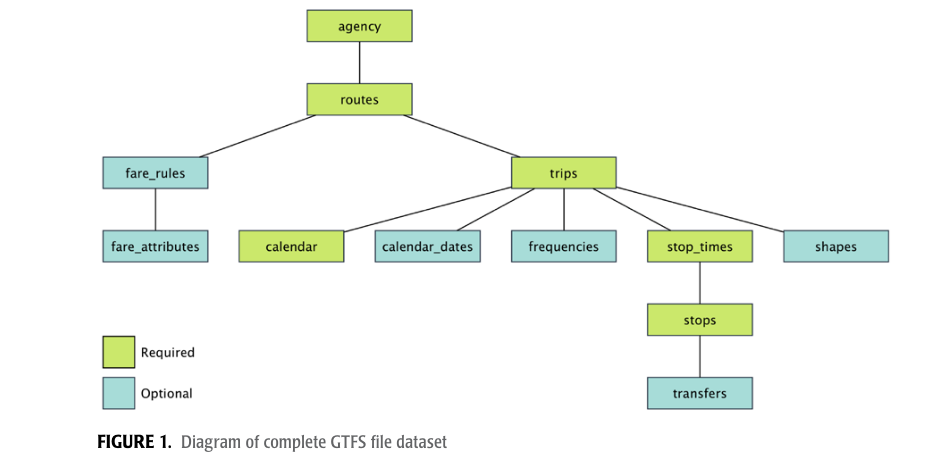
\includegraphics[width=0.85\textwidth]{img/Cap3/DiagramCompleteDataSetGTFS.png}
   \caption[Estructura relacional de archivos \gtfs{}]{Diagrama de la estructura
   relacional de los archivos que componen el estándar \gtfs{}.}
   \label{fig:gtfs-estructura}
   \fuentefigura{\cite{fortin2016innovative}, p.~21.}
 \end{figure}

% -----------------------------------------------------------------------
\subsection{Eficiencia Urbana}
\label{subsec:eficiencia-urbana}
% -----------------------------------------------------------------------
 
\subsubsection{Eficiencia Topológica y Caminos Mínimos}
\label{subsubsec:eficiencia-topologica}
 
La eficiencia de una red de transporte se entiende, en su dimensión topológica, como
la capacidad del sistema para conectar cualquier par de puntos origen-destino a
través del camino de menor costo posible ---medido en términos de tiempo de viaje,
número de transbordos o distancia recorrida---. Esta propiedad es directamente
computable sobre el grafo de la red mediante algoritmos de caminos mínimos, lo que
la convierte en una de las métricas más operativas del análisis propuesto en este
trabajo.
 
\cite{fortin2016innovative} plantean que los indicadores derivados de la teoría de grafos
---como el \termino{índice alfa} (grado de ciclicidad), el \termino{índice gamma}
(grado de conectividad) y el \termino{índice de superposición de líneas}---
caracterizan la eficiencia del diseño de la red de manera directamente relacionada
con su topología. Sin embargo, estos autores reconocen que tales indicadores no
consideran las características únicas del transporte público, como la frecuencia de
servicio, la posibilidad de transferencias entre líneas o la variabilidad del servicio a
lo largo del día; por ello proponen complementarlos con indicadores dinámicos
derivados del modelo de grafo expandido en el tiempo construido con datos \gtfs{}.
En este modelo, la eficiencia se mide a través del camino mínimo ponderado en la
dimensión temporal, que incorpora tiempos de espera y frecuencias reales de cada
línea.
 
Mishra et al. (2012), citados por \cite{mishra2012}, introdujeron en este
contexto el concepto de \termino{índice de conectividad} de un nodo como una
medida de desempeño que va más allá de la centralidad tradicional. Este índice se
define como la suma de las potencias de conexión de todas las líneas que pasan por
un nodo, considerando características operativas como la velocidad, la capacidad, la
frecuencia, el tiempo de encabezamiento (\textit{headway}) y la distancia desde el
punto de origen. Así, la eficiencia topológica y la eficiencia operativa se integran en
una sola métrica nodal computable, que será adoptada como referencia en la
construcción de los indicadores del presente trabajo.

\subsubsection{Centralidad de Intermediación y Congestión de Rutas}
\label{subsubsec:centralidad-intermediacion}
 
La distribución de los flujos de tráfico a lo largo de la red determina, en gran medida,
su eficiencia operativa. Un sistema topológicamente bien diseñado puede resultar
ineficiente en la práctica si los flujos de demanda se concentran
desproporcionadamente sobre un subconjunto reducido de nodos o aristas, generando
congestión y tiempos de viaje superiores a los predichos por el modelo teórico.
 
\cite{batista2015} proponen abordar este problema mediante una variación
ponderada de la \termino{centralidad de intermediación} (\textit{betweenness
centrality}), en la que el grafo de la red vial es ponderado no solo por la longitud de
las aristas, sino por el número de rutas generadas por la demanda real de tráfico,
representada mediante una matriz origen-destino (\textsc{od}). En su marco teórico,
un nodo o arista de alta centralidad de intermediación es aquel que aparece con mayor
frecuencia en los caminos mínimos entre los pares origen-destino del sistema; los
nodos con esta propiedad concentran los flujos de manera natural y son, por tanto,
los primeros en colapsar ante un incremento de demanda o una perturbación. La
eficiencia urbana aumenta cuando el sistema logra redistribuir estos flujos hacia rutas
alternativas, reduciendo la dependencia de los nodos centrales y homogeneizando
la carga sobre la red.
 
Esta perspectiva es fundamental para el análisis de la red metropolitana objeto del
presente estudio: la identificación computacional de los arcos y nodos con mayor
centralidad de intermediación ponderada por la demanda permite señalar aquellos
segmentos del sistema donde las inversiones en infraestructura o las modificaciones
de rutas producirían las mayores ganancias en eficiencia global.

\subsection{La Metáfora de la Higuera y la Crisis del Sistema Radial}
\label{subsubsec:metafora-crisis}

Para comprender la urgencia de una reconfiguración topológica en la ZMVM, es útil recurrir a 
la \textbf{Metáfora de la Higuera} de Sylvia Plath: 

\citaclave{
  ``De la punta de cada rama, como si de un grueso higo morado se tratara, pendía un maravilloso futuro, señalado y rutilante. 
    Un higo era un marido y un hogar feliz e hijos y otro higo era un famoso poeta, y otro higo era un brillante profesor, y 
    otro higo era Europa y África y Sudamérica y otro higo era Constantino y Sócrates y Atila y un montón de otros amantes con 
    nombres raros y profesionales poco usuales, y otro higo era una campeona de equipo olímpico de atletismo, y más allá y por 
    encima de aquellos higos había muchos más higos que no podía identificar claramente. 
    \\
    Me vi a mí misma sentada en la bifurcación de ese árbol de higos, muriéndome de hambre sólo porque no podía decidir cuál 
    de los higos escoger. Quería todos y cada uno de ellos, pero elegir uno significaba perder el resto, y, mientras yo estaba 
    allí sentada, incapaz de decidirme, los higos empezaron a arrugarse y a tornarse negros y, uno por uno, cayeron al suelo, 
    a mis pies.''
  \cite{plath1963belljar}
}

En esta analogía, el sistema de transporte radial de la ciudad funciona como un tronco único del cual brotan diversas ramas 
(opciones de vida y movilidad). Sin embargo, la centralización operativa y la falta de conexiones transversales obligan al 
usuario a elegir una sola "rama": el centro saturado \cite{ramirez2025analisis}.

Esta estructura radial fuerza la convergencia de flujos hacia hubs críticos como Pantitlán o Indios Verdes, 
provocando que las opciones de accesibilidad en la periferia se "marchiten" por la falta de alternativas. 
El Modelo VFT propone que, para preservar la viabilidad sistémica, es imperativo crear \textbf{ramas transversales} 
(Corredores Anillares) que intercepten los flujos y reduzcan la \textbf{impedancia sistémica}, 
permitiendo una distribución equitativa de la fuerza capilar en todo el territorio.
